\documentclass[a4paper,14pt]{article}

%%% Работа с русским языком
\usepackage{cmap}					% поиск в PDF
\usepackage{mathtext} 				% русские буквы в формулах
\usepackage[T2A]{fontenc}			% кодировка
\usepackage[utf8]{inputenc}			% кодировка исходного текста
\usepackage[english,russian]{babel}	% локализация и переносы
\usepackage{indentfirst}
\frenchspacing

\newcommand{\vyp}{\ensuremath{\hookrightarrow}}
\renewcommand{\epsilon}{\ensuremath{\varepsilon}}
\renewcommand{\phi}{\ensuremath{\varphi}}
\renewcommand{\kappa}{\ensuremath{\varkappa}}
\renewcommand{\le}{\ensuremath{\leqslant}}
\renewcommand{\leq}{\ensuremath{\leqslant}}
\renewcommand{\ge}{\ensuremath{\geqslant}}
\renewcommand{\geq}{\ensuremath{\geqslant}}
\renewcommand{\emptyset}{\varnothing}
\newcommand{\Ra}{\ensuremath{\Rightarrow}}
\newcommand{\ra}{\ensuremath{\rightarrow}}
\newcommand{\LRa}{\ensuremath{\Leftrightarrow}}
\newcommand{\tbf}{\textbf}
\newcommand{\ov}{\ensuremath{\overline}}
\newcommand{\CC}{\ensuremath{\mathbb{C}}}
\newcommand{\RR}{\ensuremath{\mathbb{R}}}
\newcommand{\NN}{\ensuremath{\mathbb{N}}}
\newcommand{\QQ}{\ensuremath{\mathbb{Q}}}
\newcommand{\ZZ}{\ensuremath{\mathbb{Z}}}

%%% Дополнительная работа с математикой
\usepackage{amsmath,amsfonts,amssymb,amsthm,mathtools} % AMS
\usepackage{icomma} % "Умная" запятая: $0,2$ --- число, $0, 2$ --- перечисление

%% Номера формул
%\mathtoolsset{showonlyrefs=true} % Показывать номера только у тех формул, на которые есть \eqref{} в тексте.
%\usepackage{leqno} % Нумереация формул слева

%% Свои команды
\DeclareMathOperator{\sgn}{\mathop{sgn}}

%% Перенос знаков в формулах (по Львовскому)
\newcommand*{\hm}[1]{#1\nobreak\discretionary{}
{\hbox{$\mathsurround=0pt #1$}}{}}



%%% Работа с картинками
\usepackage{graphicx}  % Для вставки рисунков
\graphicspath{{images/}{images2/}}  % папки с картинками
\setlength\fboxsep{3pt} % Отступ рамки \fbox{} от рисунка
\setlength\fboxrule{1pt} % Толщина линий рамки \fbox{}
\usepackage{wrapfig} % Обтекание рисунков текстом

%%% Работа с таблицами
\usepackage{array,tabularx,tabulary,booktabs} % Дополнительная работа с таблицами
\usepackage{longtable}  % Длинные таблицы
\usepackage{multirow} % Слияние строк в таблице

%%% Теоремы
\theoremstyle{plain} % Это стиль по умолчанию, его можно не переопределять.
\newtheorem{theorem}{Теорема}[section]
\newtheorem{proposition}[theorem]{Утверждение}
 
\theoremstyle{definition} % "Определение"
\newtheorem{corollary}{Следствие}[theorem]
\newtheorem{problem}{Задача}[section]
 
\theoremstyle{remark} % "Примечание"
\newtheorem*{nonum}{Решение}

%%% Программирование
\usepackage{etoolbox} % логические операторы

%%% Страница
\usepackage{extsizes} % Возможность сделать 14-й шрифт
\usepackage{geometry} % Простой способ задавать поля
	\geometry{top=20mm}
	\geometry{bottom=20mm}
	\geometry{left=5mm}
	\geometry{right=15mm}
 %
\usepackage{fancyhdr} % Колонтитулы
 	\pagestyle{fancy}
 	\renewcommand{\headrulewidth}{1pt}  % Толщина линейки, отчеркивающей верхний колонтитул
%\fancypagestyle{firstpage}{
	\rhead{\large{Исыпов Илья}}
%}
% 	\lfoot{Нижний левый}
% 	\rfoot{\large{Рябых Владислав, Б05-905}}
% 	\rhead{Верхний правый]}
% 	\chead{Верхний в центре}
 	\lhead{\large{Рябых Владислав}}
%	\cfoot{Нижний в центре} % По умолчанию здесь номер страницы

\usepackage{setspace} % Интерлиньяж
\onehalfspacing % Интерлиньяж 1.5
%\doublespacing % Интерлиньяж 2
%\singlespacing % Интерлиньяж 1

\usepackage{lastpage} % Узнать, сколько всего страниц в документе.

\usepackage{soul} % Модификаторы начертания

\usepackage{hyperref}
\usepackage[usenames,dvipsnames,svgnames,table,rgb]{xcolor}
\hypersetup{				% Гиперссылки
    unicode=true,           % русские буквы в раздела PDF
    pdftitle={Заголовок},   % Заголовок
    pdfauthor={Автор},      % Автор
    pdfsubject={Тема},      % Тема
    pdfcreator={Создатель}, % Создатель
    pdfproducer={Производитель}, % Производитель
    pdfkeywords={keyword1} {key2} {key3}, % Ключевые слова
    colorlinks=true,       	% false: ссылки в рамках; true: цветные ссылки
    linkcolor=red,          % внутренние ссылки
    citecolor=black,        % на библиографию
    filecolor=magenta,      % на файлы
    urlcolor=cyan           % на URL
}

\usepackage{csquotes} % Еще инструменты для ссылок

%\usepackage[style=authoryear,maxcitenames=2,backend=biber,sorting=nty]{biblatex}

\usepackage{multicol} % Несколько колонок

\usepackage{tikz} % Работа с графикой
\usepackage{pgfplots}
\usepackage{pgfplotstable}

\usepackage{caption}
\long\def\comment{}
\setlength{\abovecaptionskip}{7pt}
\setlength{\belowcaptionskip}{7pt}


\begin{document}
\author{Рябых Владислав и Исыпов Илья, Б05-905}
\title{\tbf{3.3.4. Эффект Холла в полупроводниках.}}
\maketitle

\tbf{Цель работы:} измерение подвижности и концентрации носителей заряда в полупроводниках.

\tbf{В работе используются:} электромагнит с источником питания, амперметр, миллиамперметр, милливеберметр, реостат, цифровой вольтметр, источник питания (1,5~В), образцы легированного германия.


\section*{Теория}

Суть эффекта холла состоит в следующем. Пусть через однородную пластину металла вдоль оси $x$ течет ток $I$.

\begin{wrapfigure}{l}{0.44\textwidth}
	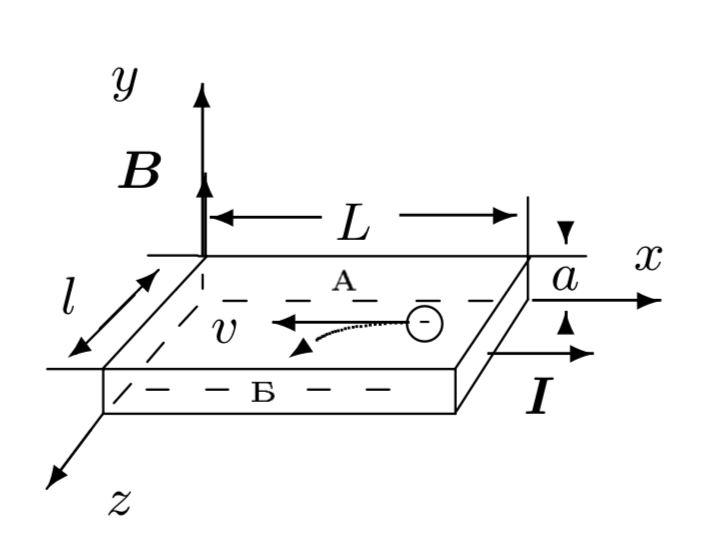
\includegraphics[width =0.36\textwidth]{theory_1.png}
	\newline
\end{wrapfigure}


Если эту пластину поместить в магнитное поле, направленное по оси $y$,то между гранями А и Б появляется разность потенциалов. В самом деле, на электрон, движущийся с скоростью $\Vec{\langle\upsilon\rangle}$ в электромагнитном поле, действует сила Лоренца:

\begin{equation}
\Vec{F_\textnormal{Л}} = -e\Vec{E} - e\Vec{\langle\upsilon\rangle}\times\Vec{B},
\label{eq1}
\end{equation}
где, e - абсолютная величина заряда электрона, $\Vec{E}$ - напряженность электрического поля, $\Vec{B}$ - индукция магнитного поля. В нашем случае сила, обусловленная слагаемым, направлена вдоль оси $z:$
$$F_B = e|\langle\Vec{\upsilon_x}\rangle|B.$$
Где $|\langle\Vec{\upsilon}\rangle| -$ средняя скорость дрейфа электрона по оси x, возникающая под действием внешнего электрического поля.
\newline
Под действием силы Электроны отклоняются к грани Б, заряжая ее отрицательно (для простоты рассматриваем только один тип носителей). На грани А накапливаются нескомпенсированные положительные заряды. Это приводит к возникновению электрического поля $E_z$, направленного от А к Б, которое действует на электроны с силой $F_E = eE_z$, направленной против силы $F_B$. В установившемся режиме сила $F_E$ уравновешивает силу $F_B$, и накопление электрических зарядов на боковых гранях пластины прекращается. Из условия равновесия $F_B = F_E$ найдём 
\begin{equation}
E_z = |\langle\upsilon_x\rangle|B.
\label{eq2}
\end{equation}
Поле $E_z$ дает вклад в общее поле $\vec{E}$, в котором движутся электроны. С полем $E_z$ связана разность потенциалов $U_{AB}$ между гранями А и Б:
\begin{equation}
U_{AB} = -E_zl = -|\langle\upsilon_x\rangle|Bl.
\label{eq3}
\end{equation}
В этом и состоит эффект Холла. Второе слагаемое в силе Лоренца \eqref{eq1}, с которым связан эффект, часто называют "холловским". 


Замечая, что сила тока
\begin{equation}
I = ne|\langle\upsilon_x\rangle|l|\cdot a,
\label{eq4}
\end{equation}
и объединяя \eqref{eq2} и \eqref{eq4}, найдем ЭДС Холла:
\begin{equation}
\mathscr{E}_x = U_{AB} = -\frac{IB}{nea} = -R_x\cdot\frac{IB}{a}.
\label{eq5}
\end{equation}
Константа $R_x$ называется постоянной Холла. Как видно из \eqref{eq5},
\begin{equation}
R_x = \frac{1}{ne}
\label{eq6}
\end{equation}
В полупроводниках, когда вклад в проводимость обусловлен и электронами и дырками, выражение для постоянной Холла имеет более сложный вид:
$$R_x = \frac{nb_e^2 - pb_p^2}{e(nb_e + pb_p)^2}$$
Если основной вклад в эффект вносит один из носителей, то для постоянной Холла можно пользоваться выражением \eqref{eq6}. Измеряя величину $R_x$, можно с помощью  \eqref{eq6} найти концентрацию носителей тока n, а по знаку возникающей между гранями А и Б разности потенциалов установить характер проводимости - электронный или дырочный


\section*{Экспериментальная установка}

\begin{center}
	\begin{figure}[bhtp]
		\centering
		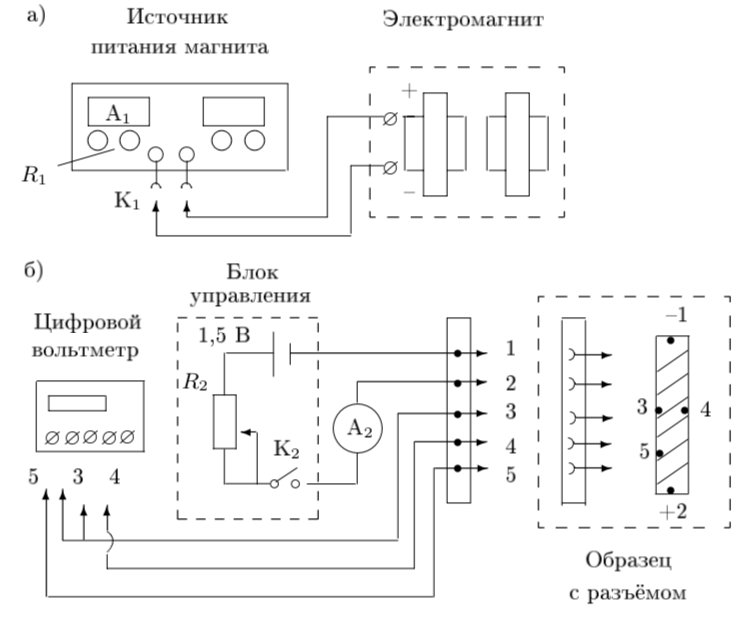
\includegraphics[width=0.8\linewidth]{scheme.png}
		\caption{Схема установки для исследования эффекта Холла в полупроводниках}
		\label{scheme}
	\end{figure}
\end{center}

	В зазоре электромагнита (рис. 1а) создаётся постоянное магнитное поле, величину которого можно менять с помощью регуляторов источника питания. Ток измеряется амперметром источника питания $A_{1}$. Разъем $K_{1}$ позволяет менять направление тока в обмотках электромагнита.

Образец из легированного германия, смонтированный в специальном держателе (рис. 1б), подключается к батарее. При замыкании ключа $K_{2}$ вдоль длинной стороны образца течет ток, величина которого регулируется реостатом $R$ и измеряется миллиамперметром $А_{2}$.

В образце с током, помещённом в зазор электромагнита, между контактами 3 и 4 возникает разность потенциалов $U_{34}$, которая измеряется с помощью цифрового вольтметра.

Контакты 3 и 4 вследствие неточности подпайки не всегда лежат на одной
эквипотенциали, и тогда напряжение между ними связано не только с эффектом
Холла, но и с омическим падением напряжения, вызванным протеканием основного тока через образец.

Измеряемая разность потенциалов при одном направлении
магнитного поля равна сумме ЭДС Холла и омического падения напряжения, а
при другом  их разности. В этом случае ЭДС Холла $\mathscr{E}_{X}$ может быть определена как половина алгебраической разности показаний вольтметра, полученных для
двух противоположных направлений магнитного поля в зазоре.

Можно исключить влияние омического падения напряжения иначе, если при каждом токе через образец измерять напряжение между точками 3 и 4 в отсутствие магнитного поля. При фиксированном токе через образец это дополнительное к ЭДС Холла напряжение $U_{0}$ остается неизменным. От него следует (с учетом
знака) отсчитывать величину ЭДС Холла: 

$$\mathscr{E}_{X} = U_{34} \pm U_{0}$$. 

При таком способе измерения нет необходимости проводить повторные измерения с противоположным направлением магнитного поля.


По знаку $\mathscr{E}_{X}$ можно определить характер проводимости - электронный или дырочный. Для этого необходимо знать направление тока в образце и направление
магнитного поля.

Измерив ток $I$ в образце и напряжение $U_{35}$ между контактами 3 и 5 в отсутствие магнитного поля, можно, зная параметры образца, рассчитать проводимость материала образца по формуле:

\begin{equation}
\sigma=\dfrac{IL_{35}}{U_{35}al}
\label{sigma}
\end{equation}

где $L_{35}$ - расстояние между контактами 3 и 5, $a$ - толщина образца, $l$ - его ширина.

\section*{Ход работы}

Запишем параметры нашей установки: 
$a = 2.2$ мм,
$L_{35} = 3.0$ мм,
$l = 2.5$ мм.

\subsection*{Калибровка электромагнита}

Определим связь между индукцией $B$ магнитного поля в зазоре электромагнита и током $I_M$ через обмотки магнита.


\begin{table}[h!]
	\centering
	\begin{tabular}{|c|c|c|c|c|c|c|c|c|c|c|}
		\hline
		$B$, мТл &20&230&395&580&748&860&940&985&1028 \\ \hline
		$I$, A
		&0	&
		0.22	&
		0.40	&
		0.60	&
		0.80	&
		1.00	&
		1.21	&
		1.40	&
		1.52	\\ \hline
	\end{tabular}
	\caption{результаты измерений}
	\label{tab1}
\end{table}

Построим график зависимости $B(I)$, см. рис \ref{gr1}

\begin{center}
	\begin{figure}[bhtp!]
		\centering
		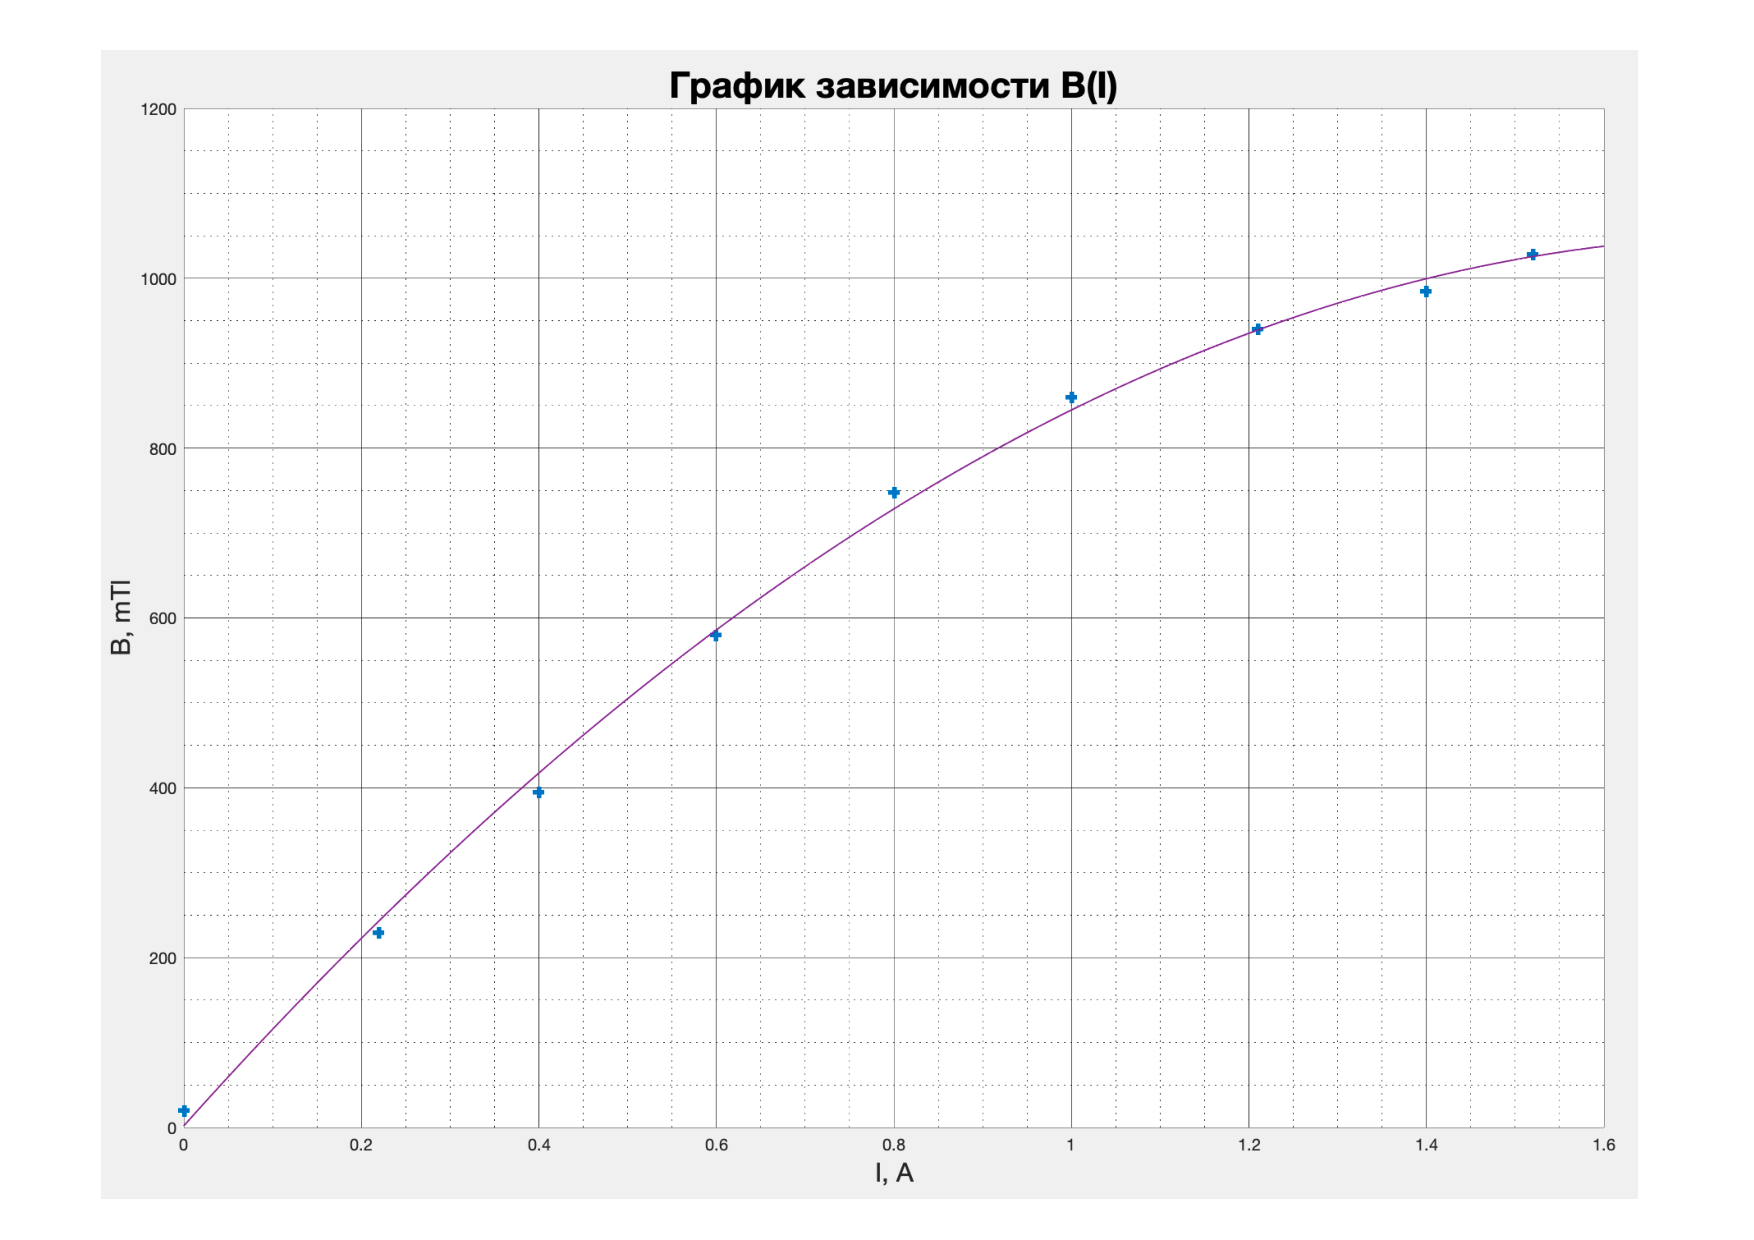
\includegraphics[width=0.8\linewidth]{gr1.pdf}
		\caption{график зависимости $B(I)$}
		\label{gr1}
	\end{figure}
\end{center}

\subsection*{Проведем измерение ЭДС Холла}

Для измерения ЭДС Холла вставим образец в зазор выключенного электромагнита и определим напряжение $U_0$ между холловскими контактами 3 и 4 при минимальном токе через образец($\simeq0,2 $ мА), включим электромагнит  и снимем зависимость напряжения $U_{34}$ от тока $I$.

\begin{table}[hbt!]
	\begin{center}
	\begin{tabular}{|c|c|c|c|c|c|c|c|c|}
		\hline
		$I$, А                         & 0  & 0.2 & 0.4 & 0.6 & 0.8 & 1   & 1.2 & 1.4 \\ \hline
		$B$, мТл                       & 20 & 230 & 395 & 580 & 748 & 860 & 940 & 985 \\ \hline
		$U_{I_0 = 0.26 \text{мА}}$, мкВ & 15 & 23  & 32  & 41  & 50  & 56  & 61  & 64  \\ \hline
			$U_{I_0 = 0.38 \text{мА}}$, мкВ & 18 & 31  & 45  & 59  & 72  & 79  & 86  & 91  \\ \hline
				$U_{I_0 = 0.50 \text{мА}}$, мкВ & 23 & 40  & 58  & 75  & 92  & 104 & 113 & 120 \\ \hline
					$U_{I_0 = 0.62 \text{мА}}$, мкВ & 28 & 49  & 71  & 94  & 114 & 131 & 140 & 148 \\ \hline
						$U_{I_0 = 0.74 \text{мА}}$, мкВ & 32 & 57  & 85  & 111 & 135 & 152 & 168 & 175 \\ \hline
							$U_{I_0 = 0.86 \text{мА}}$, мкВ & 38 & 67  & 98  & 128 & 154 & 177 & 193 & 204 \\ \hline
								$U_{I_0 = 0.99 \text{мА}}$, мкВ & 43 & 80  & 112 & 147 & 180 & 203 & 222 & 233 \\ \hline
								\end{tabular}
						\caption{результаты измерений}
					\label{tab2}
				\end{center}
			\end{table}

Построим семейство характеристик $U(B)$, см. рис \ref{gr2}. Заметим, что чем выше сила тока, тем больше $k$ -- коэффициент наклона прямой

\begin{center}
	\begin{figure}[bhtp!]
		\centering
		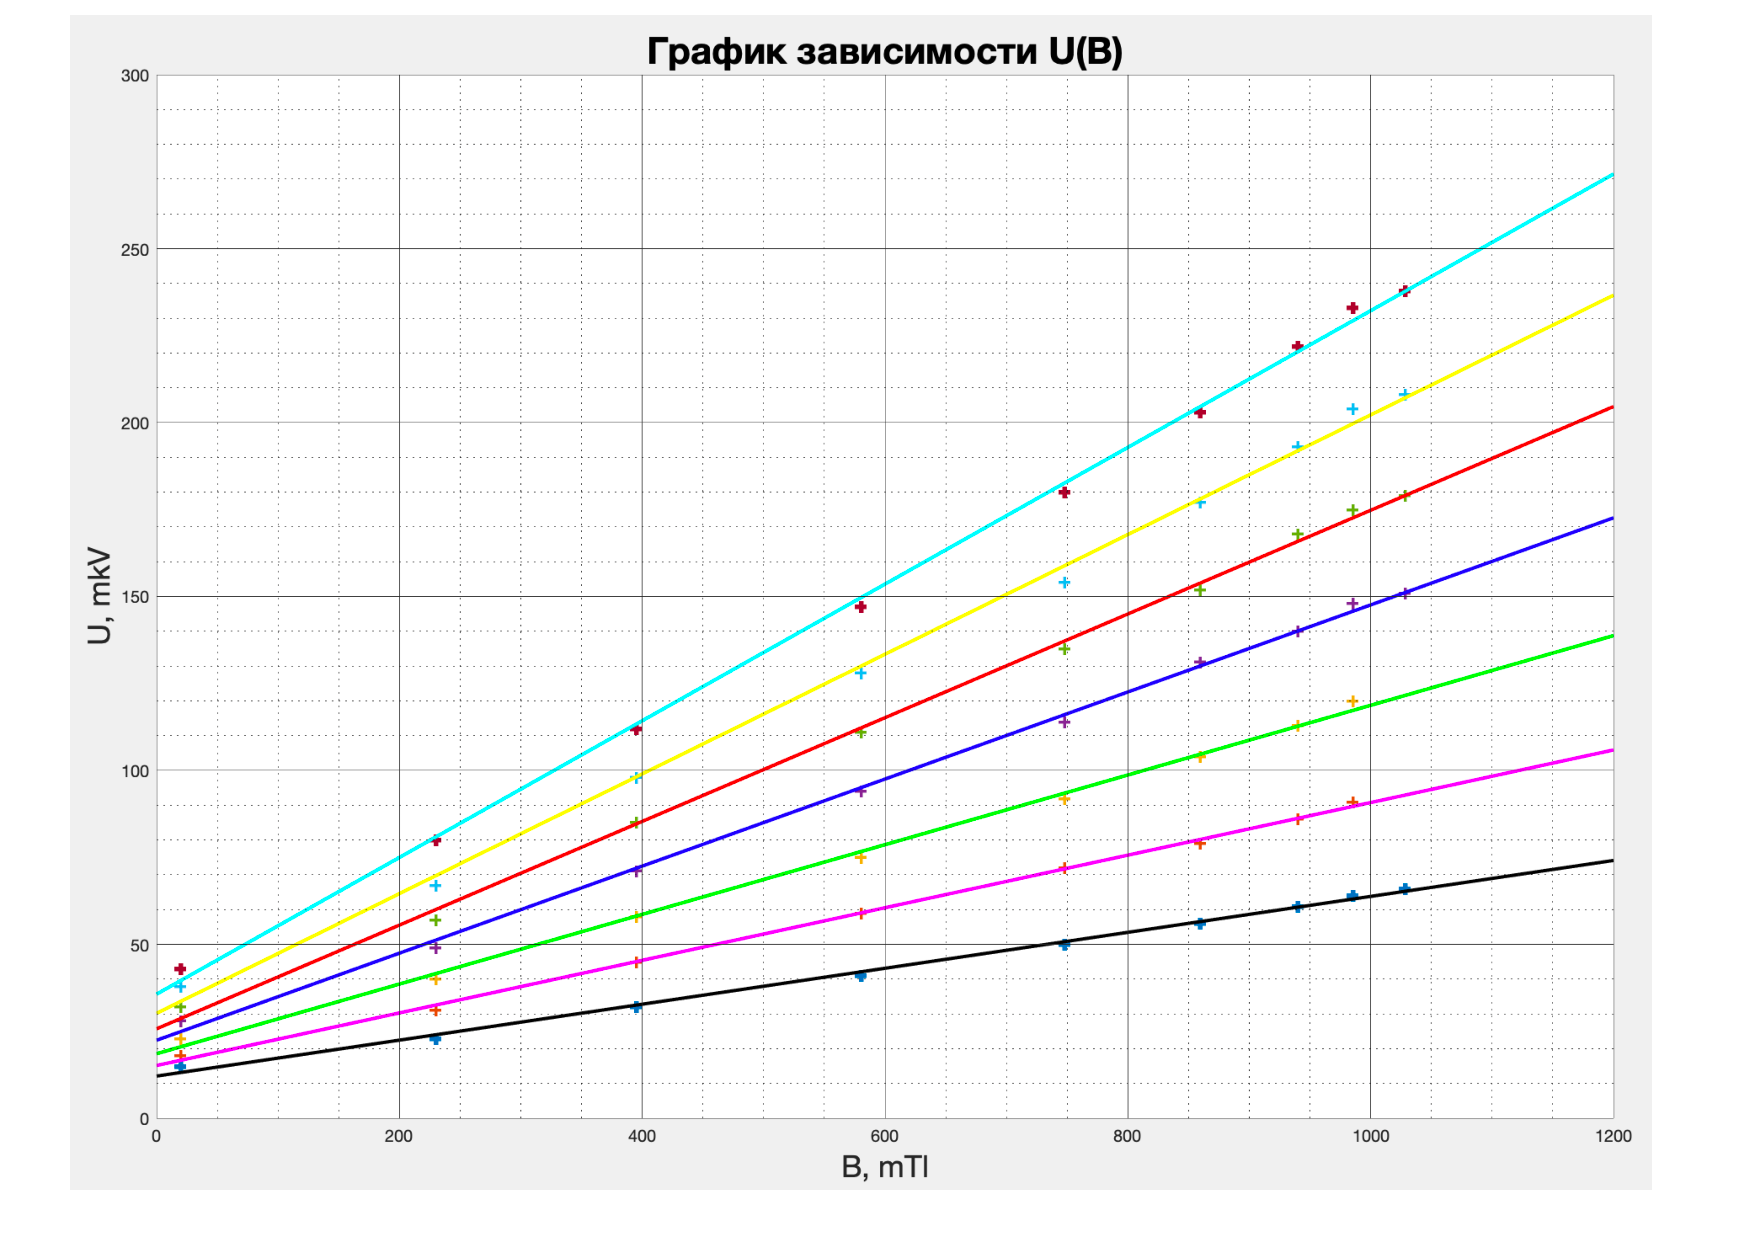
\includegraphics[width=0.7\linewidth]{gr2.pdf}
		\caption{семейство характеристик $U(B)$}
		\label{gr2}
	\end{figure}
\end{center}

Из графика \ref{gr2} получаем угловые коэффициенты $k(I) = \Delta U/\Delta B$: запишем их в таблицу \ref{tab3}

\begin{table}[hbt!]
\begin{center}
\begin{tabular}{|c|c|c|}
	\hline
	$I_0$, мА & $k, 10^{-6}\frac{\textnormal{В}}{\textnormal{Тл}}$ & $\sigma_k, , 10^{-6}\frac{\textnormal{В}}{\textnormal{Тл}}$ \\ \hline
	0.26  & 51.7                                                    & 1.7                                                           \\ \hline
	0.38  & 75.6                                                    & 2.0                                                          \\ \hline
	0.5   & 100.2                                                   & 3.4                                                          \\ \hline
	0.62  & 125.2                                                   & 4.2                                                          \\ \hline
	0.74  & 149.1                                                   & 3.7                                                          \\ \hline
	0.86  & 172                                                     & 5.8                                                          \\ \hline
	0.99  & 196.5                                                   & 6.4                                                          \\ \hline
\end{tabular}
\caption{угловые коэффициенты $k(I) = \Delta U/\Delta B$}
\label{tab3}
\end{center}
\end{table}

Построим график $k(I)$, см. рис. \ref{gr3}

\begin{center}
	\begin{figure}[bhtp!]
		\centering
		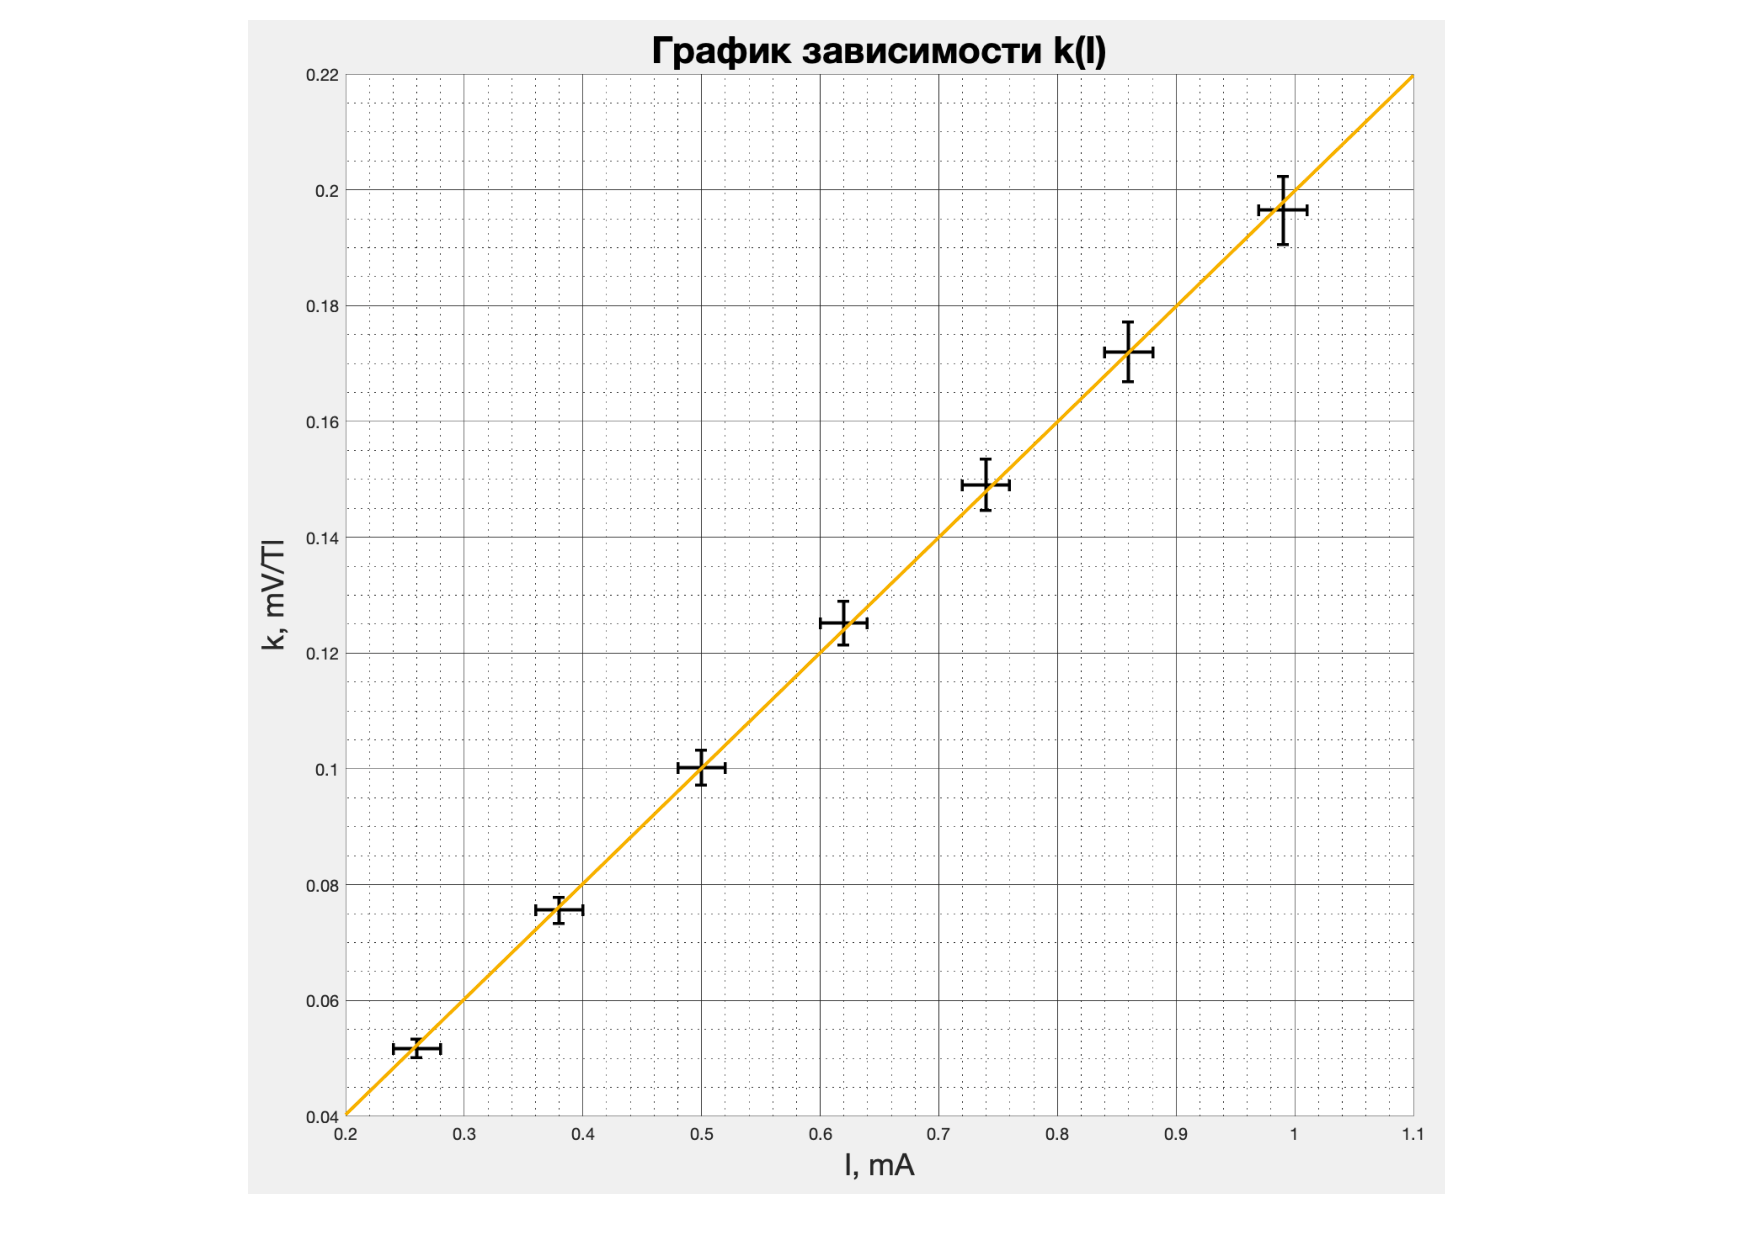
\includegraphics[width=0.6\linewidth]{gr3.pdf}
		\caption{семейство характеристик $U(B)$}
		\label{gr3}
	\end{figure}
\end{center}

По графику определим угловой коэффициент, определим величину постоянной холла $R_x$

$$R_x = -k \cdot a \approx -(7.98\pm0.69)\cdot10^{-4}\frac{\textnormal{м}^3}{\textnormal{Кл}}$$

Рассчитаем концентрацию n носителей в образце:
$$n = \frac{1}{R_xe} = (0.78\pm0.21)\cdot10^{22}\frac{\textnormal{ед}}{\textnormal{м}^3}$$

Рассчитаем удельную проводимость $\sigma$ материала образца:
$$\sigma = \frac{TL_{35}}{U_{35}al} = 148.9\frac{A}{B \cdot \textnormal{м}}$$

Вычислим подвижность носителей тока 
$$b = \frac{\sigma}{en} = (1548\pm350)\frac{\textnormal{см}^2}{B\cdot c}$$
для сравнения: табличное значение для дырок германия $b = 1820\frac{\textnormal{см}^2}{B \cdot c}$

\section*{Выводы}

	В ходе работы был исследован эффект Холла в полупроводнике-германии. Были определены такие характеристики, как постоянная Холла, концентрация холловских частиц, удельная электрическая проводимость германия и подвижность электронов-носителей заряда в нём. Результаты совпали с табличными в пределах погрешности.


\end{document}